\subsection{Relational learning across tasks for SET cards}
\label{ssec:set_exp}
\def\attr#1{{\small\texttt{#1}}}
\def\mattr#1{{\mbox{\footnotesize\texttt{#1}}}}

In this set of experiments we study
an Abstractor's ability to apply relations learned in one task to a different task.
% JDC: IS THAT THE MAIN POINT OF THIS SECTION?  SEEMS WE ADDRESSED THAT (AT LEAST IN A MORE LIMITED WAY) IN THE ARGSORT
% EXPERIMENT. WHAT SET INTRODUCES IS MULTIDIMENSIONAL (AS WELL AS HIERARHICAL?) ATTENTIONAL DEMANDS.  MAYBE WE CAN
% SAY SOMETHING LIKE:
% "...an Abstractor's ability to learn and apply relations having to do with more than one dimension, and
% hierarchical relations among those, and generalize these to different tasks."
As described in Section~\ref{ssec:set}, the game SET involves several levels of abstraction
over several dimensions
of sensory embeddings. Cards vary along the dimensions of \attr{color}, \attr{number}, \attr{pattern}, and
\attr{shape}, as shown in Figure \ref{fig_set}a). The task requires use of an AAB rule:
% JDC: I FOUND REFERENCE TO THE AAB -- AND ITS RELATIONSHIP TO SET -- CONFUSING  AT FIRST, I THOUGHT "The task"
% REFERRED TO SET, AND THAT THE AAB RULE WAS A WAY OF CHARACTERIZING IT, OR THE SAME-DIFFERENT TASK USED TO "PRE-TRAIN"
% ABSTRACTOR? OR, IS IT MEANT TO REFER TO A TASK USED TO TEST GENERALIZATION (AS SUGGESTED BY THE AAB SECTION BELOW).
% IF THAT IS SO, THEN THE DESCRIPITION THAT FOLLOWS DOESN'T SEEM QUITE RIGHT, AS IT APPEARS TO BE SPECIFIC TO SET.
% SO, EITHER NEED TO MAKE MORE EXPLICIT HOW SET CAN BE FRAMED AS AN AAB RULE, OR DEFER MENTION OF THE AAB TASK UNTIL AFTER
% DESCRIBING SET.  I ALSO THINK IT WOULD HELP TO BE MORE EXPLICIT ABOUT WHETHER THE ABSTRACTOR IS TRAINED TO FULLY
% PLAY THE SET GAME, OR JUST COMPUTATIONS THAT IT DOING SO WOULD REQUIRE.
Along each dimension, three cards in a set must either have the same or unique values. 
%As examples, if we denote this function as $f_\mattr{attr}(x_1, x_2, x_3)$
%for an attribute \attr{attr}, then the first three cards in each of the three rows of cards in Figure \ref{fig_set} 
%(reproduced below) have the following values $(f_\mattr{number}, f_\mattr{color}, f_\mattr{pattern}, f_\mattr{shape})$:
%\begin{center}
%	\begin{tabular}{cc}
%	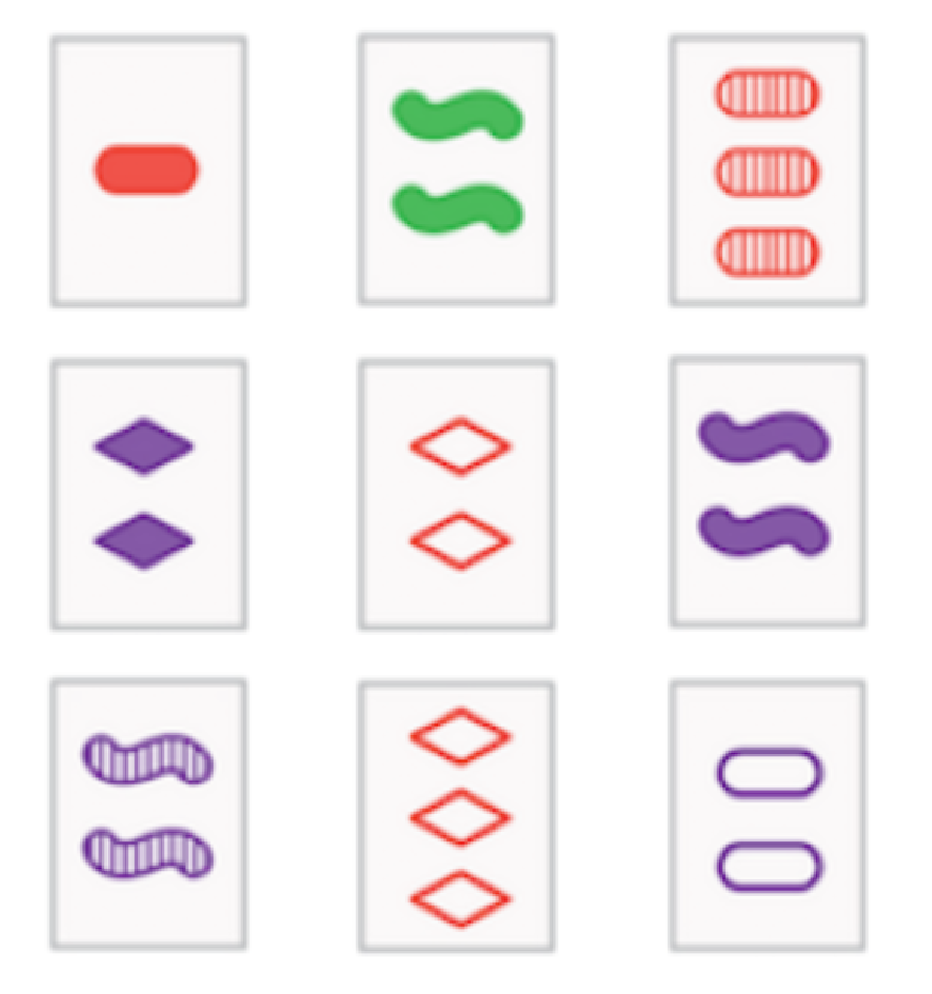
\includegraphics[width=.18\textwidth]{figures/set/set_example2}&\\[-1.05in]
%	& \renewcommand{\arraystretch}{2}
%	\begin{tabular}{c}
%     (1, 0, 0, 0) \\
%	 (1, 0, 0, 0) \\
%	 (0, 0, 0, 1) 
%	\end{tabular}
%	\end{tabular}
%\end{center}

To simulate this task we first train a convolutional neural network to process the color images 
of the cards (a full deck includes 81 cards). The CNN is trained to predict the attribute of
each card, as a multi-label classification, and then an embedding of dimension $d=32$ of 
each card is obtained as a fixed input vector.
This embedding layer uses an \MLP{} to map the convolutional feature maps into a distributed representation.
% JDC: AS AN ASIDE, DECLAN'S WORK SUGGESTS THAT, BY TRAINING END-TO-END, THE RELATIONAL BOTTLENECK CAN ACTUALLY HELP
% LEARN EMBEDDINGS THAT USE FACTORIZED REPRESENTATIONS OF ATTRIBUTES, MAKING THE ATTENTIONAL TASK "EASIER"

\subtask{Same/Different task} We train an Abstractor on a Same/Different task
in which, for a training set of pairs of cards, the Abstractor predicts whether the cards are
the same or different in each of the four attributes. The Abstractor is trained with 
four relational cross-attention heads on this task.
% JDC: THIS SEEMS LIKE A SUBSET OF SET, RATHER THAN THE GAME ITSELF.  NOT CLEAR FROM THE TEXT THAT THIS IS USED
% FOR PRE-TRAINING (AS EXPLAINED IN THE FIGURE CAPTION).

\begin{figure}[t!]
	\begin{center}
	\begin{tabular}{cc}
		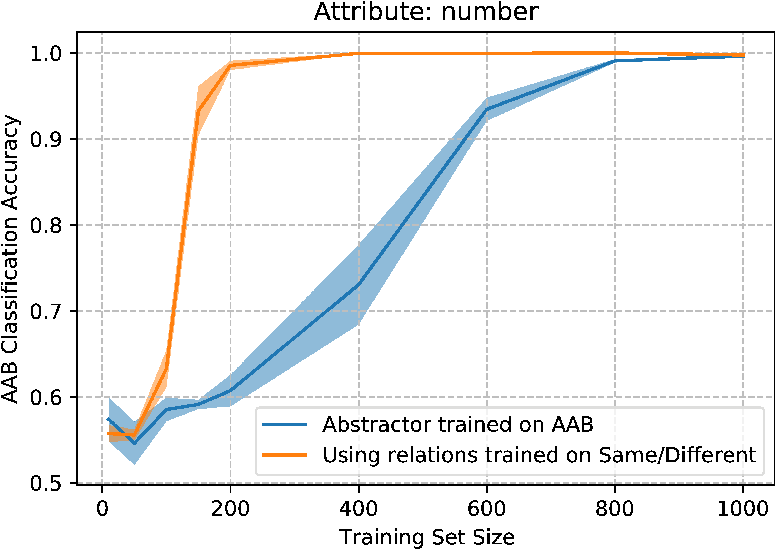
\includegraphics[width=.42\textwidth]{figures/set/AAB_same_different_number-crop} &
		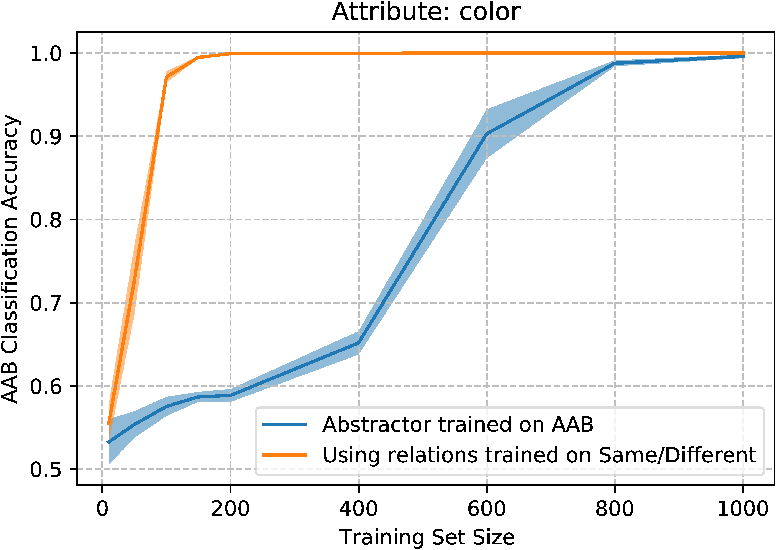
\includegraphics[width=.42\textwidth]{figures/set/AAB_same_different_color-crop} \\
		&\\
		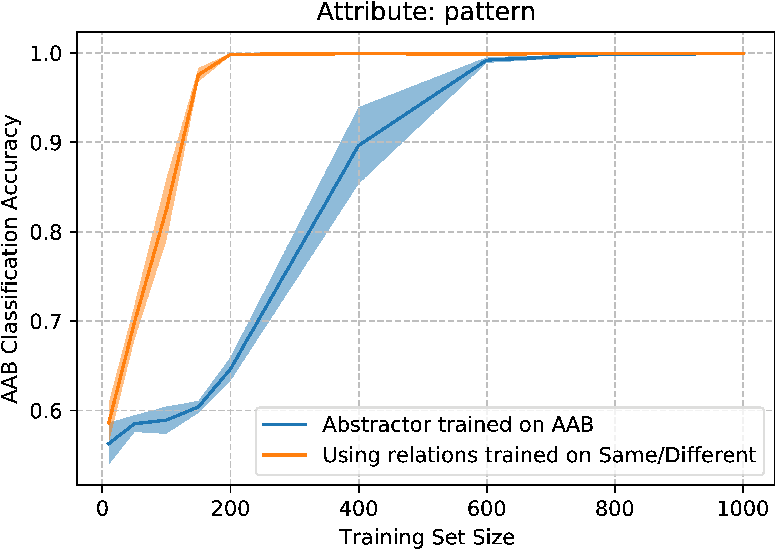
\includegraphics[width=.42\textwidth]{figures/set/AAB_same_different_pattern-crop} &
		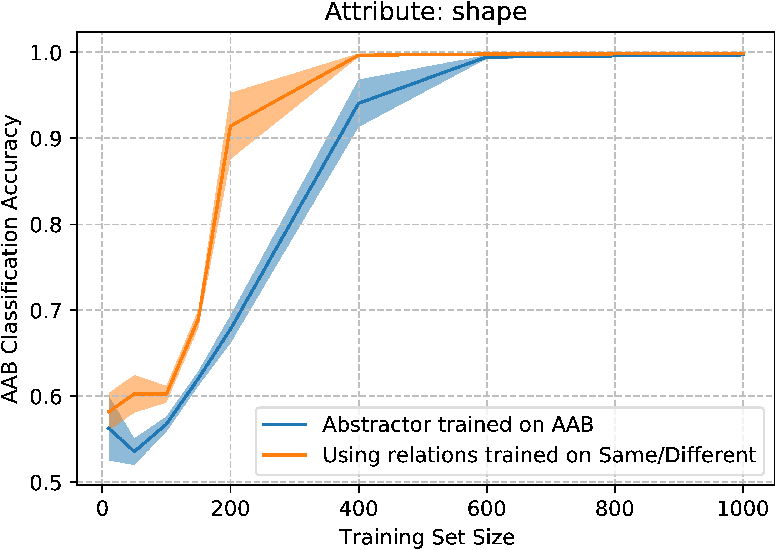
\includegraphics[width=.42\textwidth]{figures/set/AAB_same_different_shape-crop}
	\end{tabular}
	\caption{Learning curves on the SET relation learning task for all four attributes: \mattr{number}, \mattr{color},
		\mattr{pattern}, and \mattr{shape}.  An Abstractor model was first trained on the Same/Different task, as a multi-label classification task across all four attributes, using four relational cross-attention heads. The input to model is embeddings from a convolutional neural network trained on images. Two Abstractors were then trained: an Abstractor was trained from scratch on the AAB task, and another Abstractor was trained but with the relational cross attention heads initialized and fixed to be those learned in the Same/Different task--only the \MLP to classify the abstract states was trained. The lines indicate the mean AAB classification accuracy over 10 trials for that training set size, and the shaded region indicates the standard error of the mean.}
	\label{fig:aab_learning_curves}
    \end{center}
\end{figure}

% JDC: NOTE CLEAR WHAT THE STATUS OF THIS TASK IS -- A TEST OF GENERALIZATION?  MORE GENERALLY, I THINK IT WOULD HELP
% TO HAVE THE OVERALL STRATEGY LAYED OUT IN A BIT MORE DETAIL ABOVE, INCLUDING HOW THIS ALL RELATES TO THE FULL GAME
% OF SET.
\subtask{AAB task} Next, we train Abstractors separately for each of the four attributes.
Here the task is to predict whether an input triple of cards is valid for that attribute. 
If the triple forms an AAB pattern, the class label is zero; if the triple forms an ABC 
pattern or an AAA pattern, the class label is one. For each attribute we train 
two different Abstractors---the first is trained from scratch, and includes the learning 
of four new relational cross attention heads. The second Abstractor is 
initialized so that the attention heads are given by the Abstractor learned for the 
Same/Different task.
Thus, only the \MLP{} used to classify the abstract state $A=(a_1, a_2, a_3)$ is learned for this task.

\subtask{Evaluation} We evaluate learning curves on the AAB task for each 
model and attribute, for training set sizes ranging from $10$ triples to $800$ sequences in increments of $80$. For each training set size we run 10 trials. Each trial consists of training a model on a dataset of the corresponding size for 50 epochs. The classification accuracy is evaluated on an independent test sample of $500$ triples of card images. The results are shown in Figure~\ref{fig:aab_learning_curves}.

